%! TEX root = intro-optimization/main.tex
\chapter{Linear programming} % (fold)
\label{sec:Linear programming}
\includegraphics[scale=0.5]{figures/1696778670}
\section{General, standard form and augmented form linear programs} % (fold)
\label{sec:General, standard form and augmented form linear programs}

The most general form of a linear program is the following optimization problem.

\begin{align*}
  \min\, &f(x) = cx\\
  \text{s.t.}\, & Ax\ge b, x \in \mathbb{R}^{n}
.\end{align*}, for matrices \( A \in \mathbb{R}^{m \times n}\), row vector
\(c \in \mathbb{R}^{ 1\times  n} \).

\( m, n \) are called as the \textbf{number of variables} and the \textbf{number
of constraints} of the problem, respectively.

e.g. $\min f(x)=5x_{1}-6x_{2}+3x_{3}$ s.t. $8x_{1}+6x_{2}+6x_{3}=5$, $3x_{1}-2x_{2}+7x_{3}\geq 7$ and $x_{1},x_{2},x_{3}\geq 0$ has

\renewcommand\arraystretch{1.3}

\[
  [A|b]=\mleft[
  \begin{array}{ccc|c}
8 & 6 & 6 & 5 \\
-8 & -6 & -6 & -5 \\
3 & -2 & 7 & 7 \\
1 &  &  & 0 \\
 & 1 &  & 0 \\
	 &  & 1 & 0 \\
   \end{array}
   \mright], c=\begin{bmatrix}
5 & -6 & 3
\end{bmatrix}
\] (omited entries are \( 0 \))

As one can see, general form linear programs can model many different types of
constraints, like regular inequalities, equalities, and non-negative
requirements.

However, we will focus on solving a restricted form of the general problem, and
provide one a method to convert from any arbitrary general problem to a
restricted problem.

\begin{definition}
  A \textbf{standard form linear program} (SFLP) is an optimization problem in the
  form:
  \begin{align*}
  \min\, &f(x) = cx\\
  \text{s.t.}\, & Ax\ge b, x \ge  0
  .\end{align*}

  An \textbf{augmented form linear program} (AFLP) is an optimization problem in the
  form:
  \begin{align*}
  \min\, &f(x) = cx\\
  \text{s.t.}\, & Ax=  b, x \ge  0
  .\end{align*}
\end{definition}

To convert from the augmented form of a linear program to the standard form, one
can use the duplication trick as the above example, or even better, introduce a
new variable for each constraint. Such variables are called \textbf{slack
variables}.

\begin{align*}
  z &= \begin{bmatrix} x \\ y \end{bmatrix} \in \mathbb{R}^{n + m}\\
  A' &= \begin{bmatrix} A & I_{m} \end{bmatrix} \in \mathbb{R}^{m \times (n +
  m)}\\
    Ax \ge b &\iff y = b - Ax \ge  0\\
     &\iff  z \ge 0 \text{ and } Az = b
.\end{align*}, and
\begin{align*}
  &c' = \begin{bmatrix} c & 0_{m} \end{bmatrix} \in \mathbb{R}^{n + m}\\
  \implies f(x) &= cx = c'z = g(z)
.\end{align*}

Hence, the SFLP is equivalent to the following AFLP

  \begin{align*}
  \min\, &g(z) = c'z\\
  \text{s.t.}\, & A'z=  b, z \ge  0
  .\end{align*}

Converting from a general linear program to an SFLP is not as straightforward.
For every unbounded variables \( x^{i} \), let \( x^{i} = y^{i} - z^{i} \) for
some non-negative \( y^{i}, z^{i} \)
Then, the general problem is equivalent to the following SFLP

\begin{align*}
  \min\,&g(x') = c'x'\\
  \text{s.t.}\,& A'x' \ge  b, x' \ge  0
.\end{align*}, with 
\begin{align*}
  x' &= \begin{bmatrix} y \\ z \end{bmatrix} \in \mathbb{R}^{2n}\\
  A' & = \begin{bmatrix} A & -A \end{bmatrix} \in \mathbb{R}^{m \times  2n}\\
  c' &= \begin{bmatrix} c & -c \end{bmatrix} \in \mathbb{R}^{1 \times  2n} 
.\end{align*}.

Of course, this is the general case. In practice, one would want to minimize the
number of constraints and variables to make thing much easier to handle, by
utilizing "prebounded" and "already-slack" variables in the problem.
% section General, standard form and augmented form linear programs (end)

\section{Convex polyhedra} % (fold)
\label{sec:Convex polyhedra}

Let \( S \) be a subset of \( \mathbb{R}^{n} \). By convention, when we say "\(
S\) is open/closed/etc.", or talking about the boundary, closure, etc. of \( S
\), we refer to these topological concept with relative to the Euclidean
topology \( \mathbb{R}^{n} \). However, when one adds the \textit{relatively}
prefix, e.g. \( S \) is relatively open, without mentioning an explicit
topological space, that topological space is implicitly considered to be
generated from the metric space of \( \operatorname{aff} S  \), the
\textit{affine hull} of \( S \), equipped with the standard Euclidean norm.

For example, consider \( S = (-1, 1) \), then \( S \) is open (and not closed)
wrt \( \mathbb{R}
\), and both relatively open and closed wrt itself. However, since the affine
hull of \( S \) is \( \mathbb{R} \), we can not say that \( S \) is relatively
closed (without the "wrt" clause).

Consider the \( \mathbb{R}^3  \) space. The disk \( D = \{(x, y, 0), x^2+y^2\le
1\}   \), is closed wrt \( \mathbb{R}^3  \), but open in \( \mathbb{R}^2\times
\{0\}   \). The latter is the affine hull of \( D \), therefore we say that \( D
\) is relatively open.

\begin{theorem}
  If a set \( D \) is relatively closed, then \( D \) is closed.
\end{theorem}

For example, consider a hyperplane in higher dimensions. The hyperplane is
trivially relatively closed, since it is its own affine hull.

\begin{proof}
  Let \( A = \operatorname{aff} D \), \( D_{1} = A \setminus D, D_{2} =
  \mathbb{R}^{n} \setminus D \). We have \( D_{1} \subseteq D_{2} \) and \(
  A^{c} \subseteq D_{2} \).

  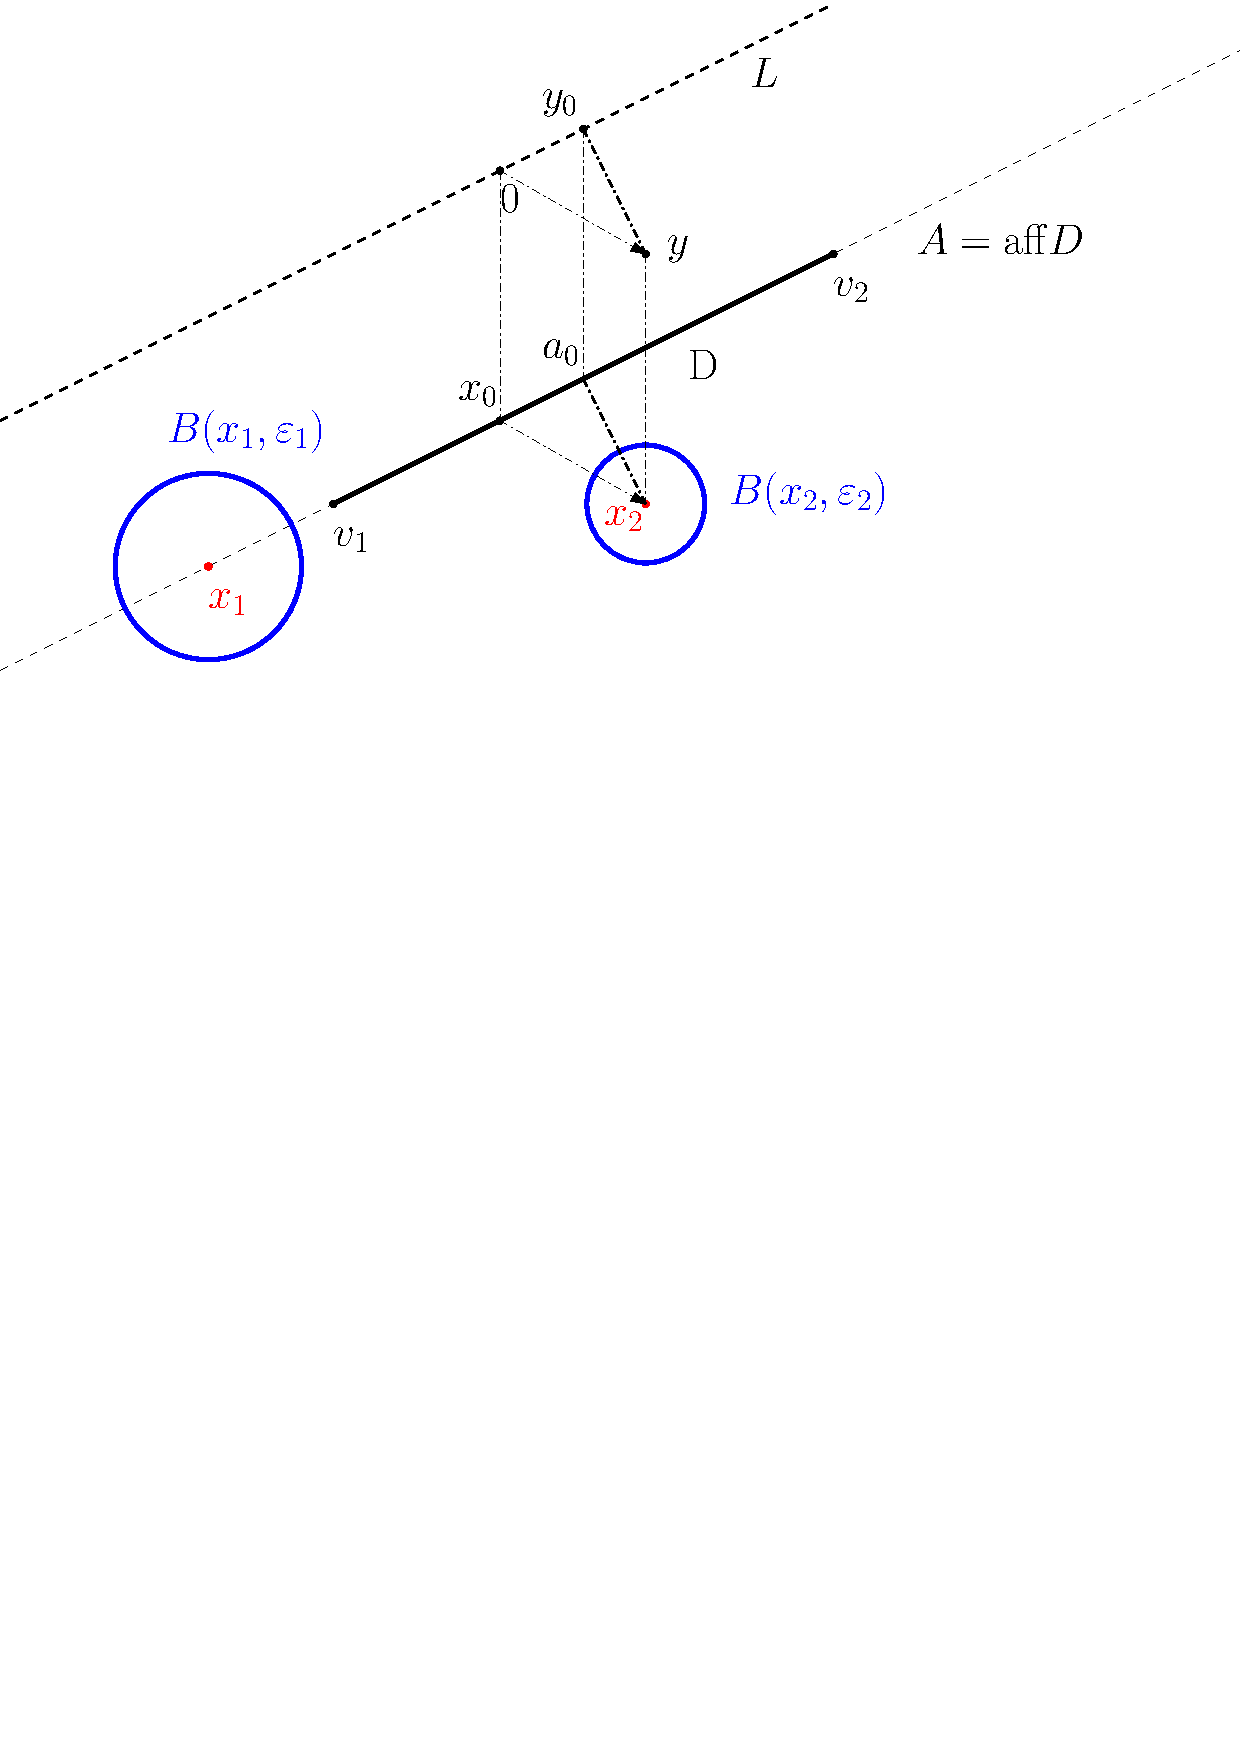
\includegraphics[scale=0.5]{figures/a}
  

  Then, \( D_{1} \) is relatively open. Let \( x \) be a point in \( D_{2} \).

  If \( x \in A \) (denoted as \( x_{1} \) in the figure above),
  then \( x \in A \). Then every neighborhood \( B_{A}(x,
  \varepsilon) \) of \( x \) is in \( D_{1} \), since \( D_{1} \) is open. Now
  consider \( y \in B(x, \varepsilon) \), then either \( y \in A \), implying \(
  y \in B_{A}(x, \varepsilon) \subseteq D_{1} \subseteq D_{2}\) or \( y \in
  A^{c} \subseteq D_{2} \). Hence, in all cases \( y \in D_{2} \), therefore \(
  B(x, \varepsilon) \subseteq D_{2}\).

  If \( x \in A^{c} \) (denoted as \( x_{2} \) in the figure above)
  and assuming \( A = x_{0} + L \) for some linear space \(
  L\). Then, we will prove that there exists \( \varepsilon > 0 \) such that \(
  d(x, a) < \varepsilon\) for all \( a \in A \). Intuitively, the distance from
  \( x \) to \( A \) is one such value for \( \varepsilon \).
  Making thing rigorous,
  let \( u = a - x_{0} \) and \( y = x - x_{0} \), then \( u \in L \). We will
  project \( x \) to \( A \), or equivalently, \( y \) to \( L \). Denote this
  projection as \( y_{0} \). Then, \( y \neq  y_{0} \) and \( d(y, y_{0}) > 0
  \). Pick \( \varepsilon = \frac{1}{2} d(y, y_{0}) \), then \( d(x, a) >
  \varepsilon \) , for every \( a \in A \), which means \( B(x, \varepsilon)
  \cap A = \varnothing \) or \( B(x, \varepsilon) \subseteq A^{c} \subseteq
  D_{2} \).

  In all cases, there exists \( \varepsilon > 0 \) such that \( B(x,
  \varepsilon) \in D_{2} \). Hence, \( D_{2} \) is open and \( D \) is closed.
\end{proof}



\subsection{Hyperplanes and related theorems} % (fold)
\label{sub:Hyperplanes and related theorems}

Consider the feasible for the above problem: \( D = \{x, Ax\ge b\}   \). Then,
one can see that \( D \) is the intersection of sets \( H_{i}=\{x, A^{i}x \ge
b^{i}\}   \) for \( i \) ranging from \( 1 \) to \( m \).

Now, we will have some names for these sets.

\begin{definition}
  A \textbf{hyperplane} is a set \( H \) in the form of \( H = \{x, ax =
  \alpha\}   \). \( H \) splits the whole space into two open sets, which are
  called \textbf{open half-spaces}: \( H_{1} = \{x, ax > b\}   \) and \( H_{2}
  = {x, ax < b} \). There are also \textbf{closed half spaces} \( H_{3} = H_{1}
  \cup H =
  \{x, ax \ge  b\}  \) and \( H_{4} = H_{2} \cup  H = \{x, ax \le  b\}   \). The
  vector \( a^{T} \) is a \textbf{normal} of \( H \).

  Let \( S \subseteq \mathbb{R}^{n} \) and \( x_{0} \in S \). Then, a hyperplane
  \( H = \{x, ax = \alpha\}   \) is a \textbf{supporting hyperplane} of \( S \)
  at \( x_{0} \) iff \( x_{0} \in H \) and either \( S \subseteq H_{1} \) or \(
  S \subseteq H_{2}\), with \( H_{1}, H_{2} \) being the closed half-spaces
  bounded by \( H \).

  Let \( A, B \) be two subsets of \( \mathbb{R}^{n} \). Then, a hyperplane \( H
  \) \textbf{separates} \( A \) and \( B \) if and only if \( H \) splits the \(
  \mathbb{R}^{n}\) space into two closed half-spaces \( H_{1} \) and \( H_{2} \)
  such that \( A \subseteq H_{1} \) and \( B \subseteq H_{2} \).
\end{definition}

Before going on proving the important hyperplane theorems, we start with a
simple lemma.

\begin{lemma}
\label{lem:Existence of closest element}
  Let \( S \) be a nonempty, closed set in \( \mathbb{R}^{n} \).
  Then for every \( x_{0} \in S^{c} \), there exists some \( x_{1} \in S \)
  such that \( d(x_{0}, x_{1}) \le d(x_{0}, x), \forall x \in S \).
\end{lemma}

\begin{proof}
  Note that this is basically a minimization problem: \( \min f(x) = d(x_{0}, x), x \in
  S\), then we can use the theorems in the last chapter to prove that a GOS
  exist. We will use Theorem \ref{thr:coercive condition}, which requires \(
  f(x) \) to be (lower semi-)continuous and \( \lim_{x \to \infty} f(x) =
  +\infty \), which are both basic properties of the Euclidean norm.
\end{proof}

\begin{theorem}[Hyperplane Separation Theorem (Closed set-point variant)]
\label{thr:hst-closed-pt}
  Let \( S \) be a nonempty, convex set and denote \( S' \) be its relative
  closure: \( S' = \operatorname{relclo} S = S \cup \operatorname{relbnd} S \).
  Then for every \( x_{0} \in S'^{c} \),
  there exists some hyperplane separating \( S' \) (and therefore \( S \))
  and \( \{x_{0}\}   \).
\end{theorem}

\begin{proof}
  Let \( x_{1} \) be the closest point on \( \overline{S} \) to \( x_{0} \), denote \( d =
  (x_{1}-x_{0})^{T}\).

  Then, we will prove that the hyperplane \( H = \{x, dx = dx_{1}\}   \) is a
  supporting hyperplane of \( S \). If this is true, then it's trivial that \( H
  \) separates \( S \) and \( \{x_{0}\}   \).

  Now, we have \( dx_{0}-dx_{1}=-d^{T}d < 0 \), which means that \( x_{1} \in
  H_{1} = \{dx < dx_{1}\}   \). Hence, we need to prove that \( S \subseteq
  H_{2} = \{dx \ge  dx_{1}\}   \), or \( x \in S \implies dx \ge  dx_{1} \).

  Assuming that there is some \( x_{2} \in S \) such that \( dx_{2} < dx_{1} \).
  Consider the lerp between \( x_{2} \) and \( x_{1} \): \( x(\lambda) =
  \operatorname{lerp}(x_{2}, x_{1}, \lambda) \), which must be in \( S \) for
  every \( \lambda \in [0, 1] \)
  \begin{align*}
    x(\lambda) - x_{0} &= \operatorname{lerp}(x_{2}, x_{1}, \lambda) -
    x_{0}\\
                       &= \operatorname{lerp}(x_{2}-x_{1}, 0, \lambda) + (x_{1}
                       - x_{0})\\
                       &= \lambda(x_{2}-x_{1}) + d^{T}\\
  .\end{align*}

  \begin{align*}
    \|x(\lambda)-x_{0}\|^2 &= (\lambda(x_{2}-x_{1}) + d^{T})^{T}(\lambda(x_{2}-x_{1})
    + d^{T})\\
                           &= \|d\|^2 + 2\lambda d(x_{2}-x_{1}) + \lambda
                           ^2\|x_{2}-x_{1}\|^2\\
                           &= \|x_{1}-x_{0}\|^2 + \lambda g(\lambda)
  .\end{align*},
  with \( g(\lambda) = 2d(x_{2}-x_{1}) + \lambda \|x_{2}-x_{1}\|^2 < 0 \) for
  small \( \lambda > 0 \), which means that \( \lambda g(\lambda) < 0 \) and
  therefore \( x(\lambda) \) is closer to \( x_{0} \) than \( x_{1} \), which is
  a contradiction.
\end{proof}

\textbf{Remark. } The hyperplane constructed above is a supporting hyperplane of
\( S \) at \( x_{1} \).

\begin{corollary}
  A closed convex set \( S \) is the intersection of the closed half-spaces that
  contains \( S \).
\end{corollary}

\begin{proof}
  If \( x \in S \), then every closed half-space that contains \( S \) contains
  \( x \).

  If \( x \in S^{c} \), then there exists a supporting hyperplane separating \(
  S\) and \( \{x\}   \), which means that \( x \) could not be in the closed
  half-space that \( S \) is in.
\end{proof}


\begin{theorem}[Supporting Hyperplane Theorem]
  \label{thr:Supporting Hyperplane Theorem}
  Let \( S \) be a nonempty convex set and a point \( x_{0} \in \partial S \).
  Then, there exists a supporting hyperplane of \( S \) at \( x_{0} \).
\end{theorem}

\begin{proof}
  In every open ball \( B(x_{0}, \varepsilon_{n}) \), pick a point \( x_{n} \in
  B(x_{0}, \varepsilon_{n}) \cap  S^{c}\). Then, \( \lim_{n \to \infty} x_{n} =
  x_{0}\) if \( \varepsilon_{n} \to  0 \), which we will fix to \( \varepsilon_{n}
  = \frac{1}{n}\) for example.

  Using the previous theorem, there exists hyperplanes \( H_{n} \) separating \(
  S\) from \( \{x_{n}\}   \). Let the normal unit vector of \( H_{n} \) be \(
  d_{n} \), with the convention that \( d_{n}(x-x_{n}) \ge 0, \forall  x \in
  S \).

  Hence, \( d_{n} \) is a sequence on the compact set \( \partial B(0, 1) \),
  which means that there must be a convergent subsequence \( d_{i_{n}} \) that
  converges to \( d \).

  Since \( d_{n}(x-x_{n}) \ge 0 \) for all \( x \in S \), letting \( n = i_{m}
  \) and \( m \to  \infty \), we have \( d(x-x_{0}) \ge 0 \), and therefore \(
  H=\{x, d(x-x_{0})\ge 0\}   \) is a supporting hyperplane of \( S \).
\end{proof}

\begin{corollary}[Hyperplane Separation Theorem (Set-point variant)]
\label{cor:hst-set-pt}
  Let \( S \) be a nonempty convex set, then for every \( x \in
  (\operatorname{Int} S)^{c} \), there is a supporting hyperplane \( H \) that
  separates \( S \) and \( \{ x\}   \).
\end{corollary}

\begin{proof}
  If \( x \in \partial S \), the supporting hyperplane exists due to Theorem
  \ref{thr:Supporting Hyperplane Theorem}.

  If \( x \in \overline{S}^{c} \), then if \(\overline{S} \) is a convex set,
  there exists a supporting hyperplane of \( \overline{S} \) at \( x \), which
  is also a supporting hyperplane of \( S \) at \( x \), due to Theorem
  \ref{thr:hst-closed-pt}.

  To conclude, one would need to prove that \( \overline{S} \) is convex, using
  the following lemma.
  \begin{lemma}
    Let \( S \) be a convex set. Then \( \overline{S} \) is also a convex set.
  \end{lemma}

  \begin{proof}[Proof of lemma]
    Consider \( x \in \overline{S} \). If \( x \in S \), then there is a trivial
    sequence \( x_{n} = x \) that converges to \( x \). Otherwise, if \( x \in
    \partial S \), then every neighborhood \( B(x, \varepsilon_{n}) \) of \( x
    \) has at least some point in \( S \), which will be denoted as \( x_{n} \).
    Then, the sequence \( x_{n} \) converges to \( x \) if one let \(
    \varepsilon_{n} \to  0 \) as \( n \to  \infty \), for example \(
    \varepsilon_{n} = \frac{1}{n} \). Hence, for every \( x \in \overline{S} \),
    there is always a sequence \( x_{n} \in S \) that converges to \( x \).

    Consider a subset \( A \subseteq \overline{S} \), then there exists a
    sequence of sets \( A_{n} \) that converges to \( A \).

    Then, \( x_{n} = \mathcal{C}(A_{n}, \lambda) \to  \mathcal{C}(A, \lambda) =
    x\) because of linearity, as \( n \to  \infty \). Note that \( x_{n} \in S
    \) and we need to prove that \( x \in \overline{S} \), which is the reverse
    direction of what we've just proven above.

    If \( x \notin \overline{S} \), then there exists a neighborhood \( B(x,
    \varepsilon) \) of \( x \) that does not intersect \( \overline{S} \).
    However, that neighborhood must contain infinitely many points in the
    sequence \( x_{n} \), which is a contradiction.

    Hence, \( x \in \overline{S} \), and therefore \( \overline{S} \) closed
    under convex combination.
  \end{proof}
\end{proof}

Finally, we can prove the \textbf{Hyperplane separation theorem}.
\begin{theorem}[Hyperplane Separation Theorem]
  Let \( A, B \) be nonempty disjoint convex sets, then there exists a
  hyperplane that separates the sets.
\end{theorem}

\begin{proof}
  Consider the set \( S = S_{1} - S_{2} = \{s_{1} - s_{2},
  s_{1} \in S_{1}, s_{2} \in S_{2}\}   \).

  \( S \) is convex, since if \( x_{1}-x_{2}, y_{1}-y_{2} \in S_{1}-S_{2} \)
  (s.t. \( x_{1},y_{1} \in S_{1}, x_{2}, y_{2} \in S_{2} \)), then a convex
  combination of the two, which can be written as \(
  \operatorname{lerp}(x_{1}-x_{2},y_{1}-y_{2},\lambda) =
  \operatorname{lerp}(x_{1},y_{1},\lambda) -
  \operatorname{lerp}(x_{2},y_{2},\lambda) \in S_{1}-S_{2} \) due to the fact
  that \( operatorname{lerp}(x_{i},y_{i}, \lambda) \in S_{i} \).

  Then, using Corollary \ref{cor:hst-set-pt}, there is a hyperplane separating
  \( S_{1}-S_{2} \) and \( \{0\}   \). Moreover, there is one such hyperplane
  that passes through \( 0 \), which could be constructed by slightly modifying
  the proofs of the above theorems. Denote this hyperplane as \( H = \{x, dx \ge
  0\}   \), then we have \( dx_{1} \ge  dx_{2}, \forall x_{1} \in S_{1}, x_{2}
  \in S_{2} \).

  Let \( \alpha = \inf dS_{1}, \beta = \sup dS_{2} \), then we have \( dx_{1}
  \ge  \alpha \ge  \beta \ge dx_{2}, \forall x_{1} \in S_{1},x_{2} \in S_{2} \),
  which yields at least one separating hyperplane of \( S_{1} \) and \( S_{2}
  \): \( H'(\gamma) = \{ dx = \gamma\}   \) for any \( \gamma \in [\alpha,\beta]
  \), which is a nonempty interval.
\end{proof}

% subsection Hyperplanes and related theorems (end)

\subsection{Extreme points and recession directions} % (fold)
\label{sub:Extreme points and recession directions}

\begin{definition}
  Let \( S \) be a subset of \( \mathbb{R}^{n} \).

  If \( S \) is convex, then \( x \in S \) is an \textbf{extreme point} if and only if
  it could not be written as a strictly convex combination of a collection
  of points in
  \( S \) not containing \( x \). In other words, \( x \in S \) is an extreme
  point if for every \( y, z \in S \setminus \{x\}, w \in (0, 1)   \), we have
  \( x \neq \operatorname{lerp}(y,z,w) \).

  If a vector \( v \) satisfies, \( x + tv \in S \) for every \( x \in S \), \(
  t \ge  0\), then \( v \) is a \textbf{recession direction} of \( S \).

  A recession direction \( v \) is called a \textbf{extreme direction} if it is
  not a strictly convex combination of any collection of recession directions
  not containing directions in the form \( kv \) for scalars \( k \in \mathbb{R}
  \).
\end{definition}

Before going on proving the  \textbf{Krein-Milman Theorem}, we will look at
\textbf{faces}.

\begin{definition}
  Let \( S \) be a nonempty closed convex set. Then nonempty \( F \subseteq S \)
  is a \textbf{face} iff
  \( \exists x \in F \) is a \textit{strict convex combination} of
  finite \( A \subseteq S \), then \( A \subseteq F \).
\end{definition}

\begin{theorem}
  If \( F \) is a face of \( S \), then
  \begin{itemize}
    \item Any face \( F' \) of \( F \) is a face of \( S \).
    \item \( F \) is a closed convex set.
  \end{itemize}
\end{theorem}

\begin{proof}
  \begin{itemize}
    \item Let \( A \subseteq S \) be a finite set such that \( x =
      \mathcal{C}(A, \lambda) \in S \), then \( A \subseteq F \) because of the
      definition of faces. Using the definition once more for \( F' \), we have
      \( A \subseteq F' \), which means \( F' \) is a face of \( S \).
    \item Pick \( x \in F \) (if \( F = \varnothing \) then \( F \) is easily
      closed). Let \( L \) be the linear space corresponding to \(
      \operatorname{relclo} F = F \cup \operatorname{relbnd} F \), the relative
      closure of \( F \), since \( x, y \in F \) we have \( y - x \in F \).
      Then, one can pick \( z = x + \lambda(x - y) \) for some \( \lambda \ge 0
      \) such that \( z \in B(x, \varepsilon) \subseteq \operatorname{relint } F
      \), which means \( x \) is now a strict convex combination of \( y \) and
      \( z \). Since \( F \) is a face, \( y, z \in F \). Hence, \(
      \operatorname{relclo} F = F \), which means that \( F \) is closed.

      To make the proof more rigorous, we need to prove \( \operatorname{relclo}
      F \subseteq S\), which comes from \( S \) being a closed convex set. This
      is a rather trivial result, coming from the fact that the closure of a set
      \( F \) is the minimal closed set containing \( F \).
  \end{itemize}
\end{proof}


\begin{theorem}[Krein-Milman Theorem (Existence)]
  Let \( S \) be a nonempty, compact and convex set. Then, \( S \) has at least
  one extreme point.
\end{theorem}

\begin{proof}

  First, consider the following stronger variant of Theorem \ref{thr:Supporting
  Hyperplane Theorem}.

  \begin{lemma}[Supporting Hyperplane Theorem (Stronger variant)]
  \label{lem:Supporting Hyperplane Theorem (Stronger variant)}

  Let \( C \subseteq \mathbb{R}^{n} \) and \( x_{0} \in \operatorname{relbnd} C \).
  Then, there exists hyperplane \( H = \{x, ax = \alpha\}   \) that supports \(
  C\) at \( x_{0} \) such that \( \exists y \in C, ay \neq  \alpha \).
  \end{lemma}

  Theorem \ref{thr:Supporting Hyperplane Theorem} showed that without the last
  condition, \( H \) always exist. This last condition is the only difference
  between the basic theorem and this stronger variant.

  \begin{proof}[Proof of lemma]
    Let \( A \) be the affine hull of \( S \). Then, since \( x_{0} \in
    \operatorname{relbnd} C \), \( B(x_{0}, \varepsilon_{n}) \cap A  \) must
    intersect \( C^{c} \) at some \( x_{n} \). Then, construct the separating
    hyperplane \( H_{n} \) of \( C \) and \( x_{0} \).
  \end{proof}
  

Consider \( x \in S \). Then either

\begin{itemize}
\item \( x \in \operatorname{relbnd} S \), then there exist 
\end{itemize}

First, we prove the following lemma.

\begin{lemma}
\label{lem:xtreme-pt}
  Let \( c \) be a row vector, then the set \( F_{c}(S) = \operatorname{Argmax}
  \{cx, x \in S\}     \), is called an \textbf{exposed face} of \( S \). Then,
  every exposed face is a face.

  An extreme point of a face \( F \) of \( S \) is also an extreme point of \( S
  \).
\end{lemma}

\begin{proof}[Proof of lemma]
  If \( x = \operatorname{lerp}(y,z, w) \in F_{c} \) for some \( y,z \in S \),
  then \( cx = \operatorname{lerp}(cy, cz, w) \le \max \{cy, cz\}   \), which
  means that either \( y \) or \( z \) is a GOS of the problem. WLOG assuming \(
  cx = cy\), then we end up having \( cz = cx \). Therefore, \( y, z \in F_{c}
  \), and \( F_{c} \) is a face of \( S \).

  To prove the second statement, let \( x \) be an extreme point of \( F \).
  Assuming that there exists \( y, z \in S, \lambda \in (0, 1) \) such that \( x =
  \operatorname{lerp}(y, z, \lambda) \), then \( y, z \in F \) because of the
  definition of faces, which leads to a contradiction.
\end{proof}

Returning to the existence theorem, we will define a partial order on \(
\mathcal{A} \), the set of all nonempty exposed faces of \( S \).

If an exposed face \( F \) has one element, then it is the minimal element
in \( \mathcal{A} \),
which means that it could not be "greater" than any other exposed faces,
including other one-element exposed faces.

Otherwise, \( |F| \ge 2 \), we will construct another exposed face that is 
Returning to the existence theorem, denote
\( S_{1} = S \). Then for every \( i \), assuming \( S_{i} \) is a
nonempty face (induction hypothesis) and construct an exposed face \( S_{i+1} \) until we
have found an extreme point of \( S \):
\begin{itemize}
  \item If \( |S_{i}| = 1 \) and \( S_{i} = \{ s\}   \), then \( s \) is an
    extreme point of \( S \).
  \item If \( |S_{i}| \ge  2 \), then pick \( x, y \in S_{i}, x \neq y \). Then,
    consider the hyperplane \( H: ax = \alpha \) separating \( x \) and \( y \),
    i.e. \( ax < \alpha < ay \), which always exists. Then, let \( S_{i+1}
    \coloneqq F_{a}(S_{i}) \subset S_{i} \), which is a nonempty face that is a
    proper subset of \( S_{i} \) (since \( x \notin F_{a} \)).
\end{itemize}

Consider the family \( \mathcal{A} \) of all nonempty faces of \( S \), with the partial
order \( \subseteq \). Then, if there are only a finite amount of exposed
faces, the above procedure will have to halt at some point (Zorn's lemma).

To prove that a 
\end{proof}

\begin{theorem}[Krein-Milman Theorem]
  Let \( S \) be a nonempty, compact and convex set. Then, \( S \) is the convex
  hull of \( E(S) \), the set of its extreme points.
\end{theorem}

\begin{proof}
  Using the previous theorem, one can see that \( E(S) \) is nonempty.
  Let \( T \) be the convex hull of \( E(S) \), then one can trivially
  see that \( T \subseteq S \). Assuming there exists \( x \in T \setminus S \),
  then by the Hyperplane Separation Theorem, there is a row vector \( a \) such
  that \( \sup aT < ax \).

  Consider the face \( F_{a} = \operatorname{Argmax} \{ ax, x \in S \}   \),
  then \( T \cap  F_{a} = \varnothing \). Then, the face \( F_{a} \) would have
  an extreme point \( e' \), which means that \( e'  \notin E(S)\), which is a
  contradiction.
\end{proof}

% subsection Extreme points and recession directions (end)


\subsection{Convex polyhedra} % (fold)
\label{sub:Convex polyhedra}

\begin{definition}
  A \textbf{convex polyhedron} (plural \textit{convex polyhedra}) \( P \) is
  the intersection of finitely many closed half-spaces.

  A \textbf{convex polytope} is a bounded convex polyhedron.
\end{definition}

Then, one can write \( P \) as \( P = \{x, Ax \ge  b\}   \) for some matrix \( A
\) and row vector \( b \), with the closed half-spaces defining \( P \) being
the half-spaces \( H_{i}: A^{i}x \ge  b^{i} \).

Now, we will prove the following theorem.

\begin{theorem}[Minkowski's Theorem for Polyhedra]
\label{thr:Minkowski's Theorem for Polyhedra}
  Denote \( \operatorname{conv} V \) as the convex hull of \( V \) and \(
  \operatorname{cone} R \) as the convex cone generated by \( R \).

  Let \( P \) be a convex polyhedron, then \( P = \operatorname{conv} E(P) +
  \operatorname{cone} R(P)\), with \( E(P), R(P) \) denoting the set of all
  extreme points and extreme directions of \( P \), respectively.
\end{theorem}

\begin{proof}

If \( x \in \operatorname{conv} E(P) + \operatorname{cone} R(P) \), then it can
be easily seen that \( x \in P \).

Then, it suffices to show that \( P \subseteq \operatorname{conv} E(P)
+ \operatorname{cone} R(P) \), which is equivalent to
the fact that \( \forall x\in P, x = e_{i}\lambda^{i} + r _{j}\mu ^{j} =
e\lambda + r\mu \), with \( e \) and \( r \) being matrices with columns being
extreme points and extreme directions of \( P \), respectively. The condition
for the vectors \( \mu  \) and \( \lambda \) are \( \mu  \ge 0 \) and \(
\sum_{i} \lambda_{i} = 1 \)

Now, let
\begin{align*}
  x' &= \begin{bmatrix} x \\ 1 \end{bmatrix} \\
  A' &= \begin{bmatrix} A & -b \end{bmatrix} 
.\end{align*},
then \( Ax \ge b \) only if \( A'x' \ge  0 \).

Consider the convex cone \( C = \{x', A'x' \ge  0\}   \). If one can
prove the theorem for \( C \), which has no non-zero extreme points, then \(
\forall x' \in C, x' = r'\mu' \).

Observes that there are two types of extreme direction in \( D \), one with the
\( (n+1) \)-th component being \( 0 \) and one with that component being a
positive value, which could be normalized to \( 1 \) without loss of generality. Then, split \( r' \) according to this categorization, \( v \) is the matrix
that contains all extreme directions of the first type and \( u \) containing
extreme directions of the second type.

Then, there exists \( \lambda, \nu \ge 0 \) such that \( x' = u\lambda + v\nu \).
Moreover, \( 1 = x'^{n+1} = u^{n+1}\lambda= \sum_{i} \lambda^{i} \) since \(
u^{n+1}_{i} = 1 \) for all \( i \), since the extreme directions of the second
type is already normalized (wrt its last component).

Now, denote \( U = u^{1..n}, V = v^{1..n} \), we have \( x = x'^{1..n} =
U\lambda+V\nu \). This suggests that \( U \) and \( V \)'s columns are
extreme points and extreme directions of \( P\), respectively. This can be
trivially proven as follows
\begin{align*}
  0 \le  A'u_{i} = \begin{bmatrix} A & -b \end{bmatrix}  \begin{bmatrix} U_{i}
\\ 1 \end{bmatrix}  = AU - b
.\end{align*}
Hence, \( U \in P \). If \( U \) is a strict convex combination of two other \(
X_{1}, X_{2} \in P\), then \( u \) is a strict convex combination (wrt the same
weight) of the two extreme directions of \( C \) \( x_{1}, x_{2} \) given by:
\begin{align*}
  x_{i} = \begin{bmatrix} X_{i} \\ 1 \end{bmatrix}, i \in \{1, 2\}  
.\end{align*}, which is a contradiction to the fact that \( u \) is an extreme
direction of \( C \).
\begin{align*}
  0 \le  A'v_{i} = \begin{bmatrix} A & -b \end{bmatrix} \begin{bmatrix} V_{i} 0
\end{bmatrix}  = AV_{i}
.\end{align*}

Hence, \( V_{i} \) is a recession direction of \( P \) due to the fact that \(
\forall x \in P, t \ge  0, A(x+tV_{i}) = Ax + tAV_{i} = Ax \ge  b \). Using the
same logic as above, we can prove that \( V_{i} \) is an extreme direction of \(
P\).

\end{proof}

Therefore, the proof would be completed if we have proven the theorem for the
convex cone case:

\begin{theorem}[Minkowski's Theorem for Cones]
  Let \( C = \{x, Ax \ge  0\}   \) be a convex polyhedral cone, then \( C \) is
  contained in the conic hull of \( R(C) \), the set of its extreme directions.
\end{theorem}

\begin{proof}
  First, we prove that the set \( C_{1} = \{ x, \exists \lambda \ge 0, x =
  R\lambda\}   \) is a convex polyhedral cone, since one can use the
  \textbf{Fourier-Motzkin elimination algorithm} to turn from \( x = R\lambda,
  \lambda \ge 0 \) to \( Ax \le  0 \), which is the inequality for a polyhedral
  cone.

  Then, we say that \( (A, R) \) is a \textit{double description pair} (DDP) if
  \( Ax \le  0 \iff \exists \lambda \ge 0, x = R\lambda  \). Then, we will
  proceed to prove that \( (R^{T}, A^{T}) \) is also a DDP.

  \begin{align*}
    &R^{T}y \le 0\\
    &\iff \lambda^{T} R^{T} y \ge 0, \forall  \lambda \ge 0\\
    &\iff (R\lambda)^{T} y \ge 0, \forall  \lambda \ge 0\\
  .\end{align*}

  Let \( x = R\lambda \), then \( R^{T}y \le 0 \) iff \( x^{T}y \ge 0, \forall
  \lambda \ge 0, x = R\lambda \), or equivalently \( Ax \le  0 \). Then, the
  last statement is equivalent to \( Ax \le  0 \implies x^{T}y \le  0 \)

  To conclude this proof, we need to use \textbf{Farkas' Lemma}.

  \begin{lemma}[Farkas' Lemma]
  \label{farkas}
    \( ax \ge  0, \forall  x \) s.t. \( Ax \ge  0 \) iff \( a = yA \) for some
    row vector \( y \ge  0 \)
  \end{lemma}

  \begin{proof}[Proof of Farkas' lemma]
    If \( a = yA \), then \( ax = yAx \ge  0, \forall  Ax \ge 0 \).

    If \( ax \ge  0, \forall Ax \ge 0 \) and \( a \neq  yA, \forall  y\ge 0 \),
    then consider the set \( S = \{yA, y \ge 0\}   \). Since \( a \notin S \)
    and \( S \) is closed, using Theorem \ref{thr:hst-closed-pt}, there is a
    hyperplane \( H \) strictly separating \( S^{T} \) and \( \{ a^{T}\}   \).
    Assuming \( H = \{t, x^{T}t \ge  \alpha\}   \) satisfies \( ax  <  \alpha
    \le   \inf Sx \). Note that \( 0 \in Sx \), then \( \alpha \) must be
    non-positive. If \( \alpha < 0 \) and the hyperplane \( H' = \{ t, x^{T}t =
    0\}   \) could not separate the two sets, then there exists some \( t \in S
    \) such that \( tx < 0 \). Then, there exists \( k > 0 \) such that \( t(kx)
    < \alpha\), with \( kx \in S \), which means the original hyperplane also could
    not separate the two sets, which is a contradiction. Hence, the hyperplane
    \( H' \) could separate the two set, i.e. \( ax < 0 \le \inf Sx \). Then,
    we have \( A_{i}x \ge  0 \) for all \( i \), since \( A_{i} =
    A\mathbf{e_{i}} \in S \), with \( \mathbf{e_{i}} \) denoting the \( i \)-th
    standard basis vector, and hence \( Ax \ge 0 \). To conclude, \( ax < 0 \)
    for some \( x \) s.t. \( Ax \ge 0 \), which is another contradiction.
  \end{proof}

Continuing with the proof, we have
\begin{align*}
  &(Ax \le 0 \implies x^{T}y \le 0)\\
  &\iff(Az \ge  0 \implies z^{T}y \ge  0) \text{ (letting \( z = -x \))}\\
  &\iff \exists \lambda \ge 0,  y = \lambda A\\
  &\iff \exists  \lambda' = \lambda^{T} \ge 0, y^{T} = A^{T}\lambda'
.\end{align*}

Hence \( (R^{T}, A^{T}) \) is a DDP.

So to find \( R \), one find do Fourier-Motzkin on \( A^{T} \) to get \( R^{T}
\). Now that \( R \) exists, we have \( C = \{x, Ax \ge 0\} = \{x, \exists
\lambda \ge 0, x = -R\lambda\}  \)

Now, we will prove that \( -R_{i} \) are recession directions of \( C \).
Since \( R_{i} = R\mathbf{e_{i}}, \mathbf{e_{i}} \ge 0 \), \( R_{i} \in P \),
and \( AR_{i} \ge  0 \). Then, for every \( x \in P, t \ge 0 \), we have \( A(x
- tR_{i}) = Ax - tAR_{i} \le  0 \), which means that \( R_{i} \) is a recession
direction of \( C \). Pick columns from \( R \) to form a conical basis of \( R \)'s
column space, then this basis is able to span the recession cone of \( C \), due
to every recession direction \( d \) of \( C \) can be written as \( d =
R\lambda = R'\lambda' \) with some \( \lambda, \lambda' \ge  0 \).
\end{proof}

% subsection Convex polyhedra (end)

Now, we will consider the faces of a convex polyhedron \( P \).

\begin{theorem}
  Let \( P \) be a convex polyhedron defined by \( P = \{x, Ax \ge  b\}   \).
  
  Denote \( m \) as the number of rows in \( A \) (and \( b \)), then for
  arbitrary \( J \subseteq 1..m \), the set \( F = \{x \in P, A^{J}x = b^{J}\}
  \) is a face of \( P \).
\end{theorem}

\begin{proof}
  Assuming one has \( x \in F \), \( x = \operatorname{lerp}(y, z, \lambda) \)
  with \( \lambda \in (0, 1), y, z \in P \).

  Then, \( b^{J} = A^{J}x = \operatorname{lerp}(A^{J}y, A^{J}z, \lambda) \ge
  \operatorname{lerp}(b^{J}, b^{J}, \lambda) \). Equality only holds if \(
  A^{J}y = A^{J}z = b^{J} \), which means that \( y, z \in F \).
\end{proof}

This result may pose a question: \textit{can all faces \( F \) of \( P \) be
written in the form \( \{x, A^{J}x \ge  b\}  \) for some \( J \)?}

To answer that question, first, we will have to prove the following theorem.

\begin{theorem}
\label{thr:Faces and exposed faces in convex polyhedra}
  
\end{theorem}

The answer is yes, and it is the result of the following theorem.

\begin{theorem}
\label{thr:Face representation theorem}
  Let \( F \) be a face of the convex polyhedron \( P = \{x, Ax \ge  b\}   \). Then,
  there exists a multi-index \( J \) such that \( F = \{x, A^{J}x = b^{J}\}
  \).
\end{theorem}

\begin{proof}
  Before going on proving the theorem, we will 
  Since \( F \) is a closed convex polyhedron by itself, by
  Theorem \ref{thr:Minkowski's Theorem for Polyhedra}, \( F =
  \operatorname{conv} E + \operatorname{cone} R \),
  with \( E \) and \( R \) denoting the set of all
  extreme points and extreme directions of \( F \), respectively.

  Assuming that \( F \subseteq F(J) = \{ x \in P, A^{J}x = b^{J}\}   \), then if
  \( i \in J \), we have \( A^{i}x = b^{i} \), which is equivalent to \( A^{i}e
  = b^{i}, \forall e \in E\) and \( Ad = 0, \forall d \in R \). Let \( J \) be
  the set of such indices \( i \), then the theorem is equivalent to proving \(
  F = F(J)\).

  Note that \( F \subseteq F(J) \) due to Theorem \ref{thr:Minkowski's Theorem
  for Polyhedra}, we just need to prove that \( \nexists x \in F(J) \setminus
  F\). Assuming such \( x \) exists, then
\end{proof}
% section Convex polyhedra (end)

\section{Existence and properties of solutions of linear programs} % (fold)
\label{sec:Existence and properties of solutions of linear programs}

Firstly, since \( D = \{x\ge 0, Ax \ge  b\}   \) is a convex set (this can be
trivially seen due to the linearity of the convex combination operation) and \(
f(x)=cx\) is a convex (and a concave) function on \( \mathbb{R}^{n} \), then
every (S)LOS of the linear program is a (S)GOS.

The set \( D \) is already closed (why?) and \( f(x) \) is continuous, and hence
the problem will have a GOS if \( D \) is bounded.


% section Existence and properties of solutions of linear programs (end)

% chapter Linear programming (end)
